\documentclass[a4paper]{article} 

% Setup packages
\usepackage{booktabs}
\usepackage{graphicx}
\usepackage{multicol}
\usepackage[T1]{fontenc}
\usepackage[utf8]{inputenc}
\usepackage{fancyhdr}
\usepackage{float}
\usepackage{helvet}

\graphicspath{/}

\renewcommand{\familydefault}{\sfdefault}

\addtolength{\hoffset}{-2.25cm}
\addtolength{\textwidth}{4.5cm}
\addtolength{\voffset}{-3.25cm}
\addtolength{\textheight}{5cm}
\setlength{\parskip}{0pt}
\setlength{\parindent}{0in}

% Set the path for media
\graphicspath{ {media/} } 
\pagenumbering{arabic}

\begin{document}


\includegraphics[scale=0.2]{uva-logo.jpg} \\

\section*{Component overview for the Bluebird Data Physicalization Prototype}

The Bluebird project entails the creation of a tangible data visualization for the Lab42 building, utilizing environmental IAQ sensor data to facilitate Human Building-Interaction. Part of the Thesis and Graduation project for the Master of Science (MSc) in Information Studies (Information Systems track), created by part-time student Danny de Vries at the University of Amsterdam. \\

This document offers an outline of the expenses incurred for hardware components necessary for the prototype's development. Additionally, it presents an inventory of components already possessed by the researcher, intended for a transparent declaration of these costs within the budget allocated by the Digital Interactions Lab. \\

The invoices of all these components are included at the bottom of the document after the cost breakdown. All other hardware components and tools that are not part of this document were already in possession of the researcher. \\

The paper itself with impressions and photographs of the prototype and the models and firmware used for the physicalization can be found on GitHub under the Viszlab organization: \underline{https://github.com/viszlab}.


\section*{Thesis Project}

\begin{description}
  \item \textbf{Name:} BSc Danny de Vries (14495643)
  \item \textbf{Email:} danny.de.vries@student.uva.nl
  \item \textbf{Project:} Master Thesis (IS)
  \item \textbf{University:} University of Amsterdam (UvA)
  \item \textbf{Master:} Information Studies Information Systems (track)
  \item \textbf{Institute:} Informatics Institute
  \item \textbf{Faculty:} Faculty of Science (FNWI)
  \item \textbf{Research Group:} Digital Interactions Lab (DIL)
  \item \textbf{Supervisor(s):} Dr. H. (Hamed) Seiied Alavi PhD \& Shruti Rao Ph.D. Candidate
\end{description}

\section*{Cost Breakdown}

\textbf{Total incurred costs for this project for declaration: \textit{€64.99}}

\subsection*{Total costs:}
\begin{itemize}
    \item Costs for electronics: \textbf{€27.26}
    \item Costs for hardware: \textbf{€37.73}
\end{itemize}

\subsection*{Costs for the Electronics}

\textit{User for creation of the controller device and string pull up/down mechanism.}

\begin{itemize}
    \item 1x \texti(A) 16-channel I2C PWM-Servo Controller (PCA9685) \textit{€6.10 (A)}
    \item 7x Mini Servo (MG90S) Digital (360 continuous degrees) \textit{€17.57 (B)}
    \item 10x 500mm servo extension cables \textit{€3.59 (C)}

\end{itemize}

\subsection*{Costs for Manufacturing}

\textit{The filament was used for mounting plates, and pulleys, and attached to the wooden MDF board.}

\begin{itemize}
    \item 1x PLA spool filament yellow/green gradient: \textit{€24.99 (D)}
    \item 1x Dark green paracord 4mm: \textit{€1.49 (E)} 
    \item 1x Light green paracord 3mm: \textit{€1.38 (E)} 
    \item 1x Woven jute rope 3mm: \textit{€0.99 (E)} 
    \item 1x 122x61cm Wooden MDF board (cut to length) \textit{€6.29 (F)} 
    \item 1x Mounting Kit white 290ml \textit{€2.59 (F)} 
\end{itemize}

\section*{Invoices}

\begin{figure}[h]
    \centering
    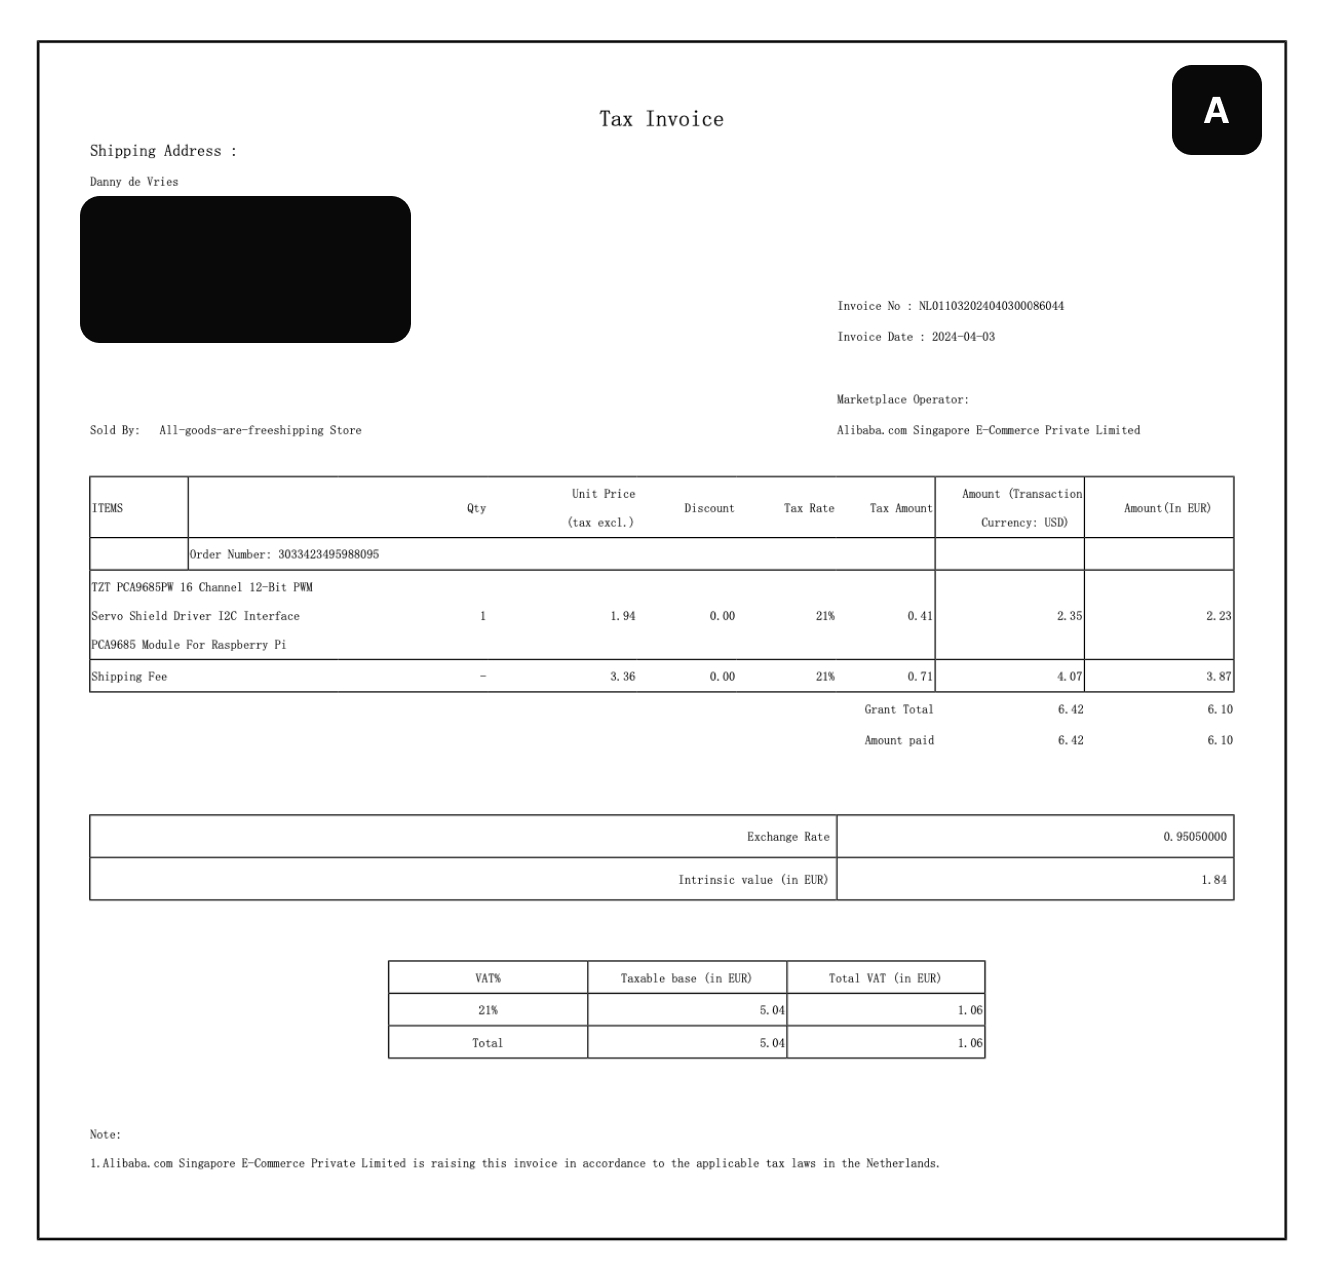
\includegraphics[width=1\textwidth]{pwm_shield.jpg}
    \caption{A) Invoice from Alibaba for the PWM shield}
    \label{fig:mesh1}
\end{figure}

\begin{figure}[h]
    \centering
    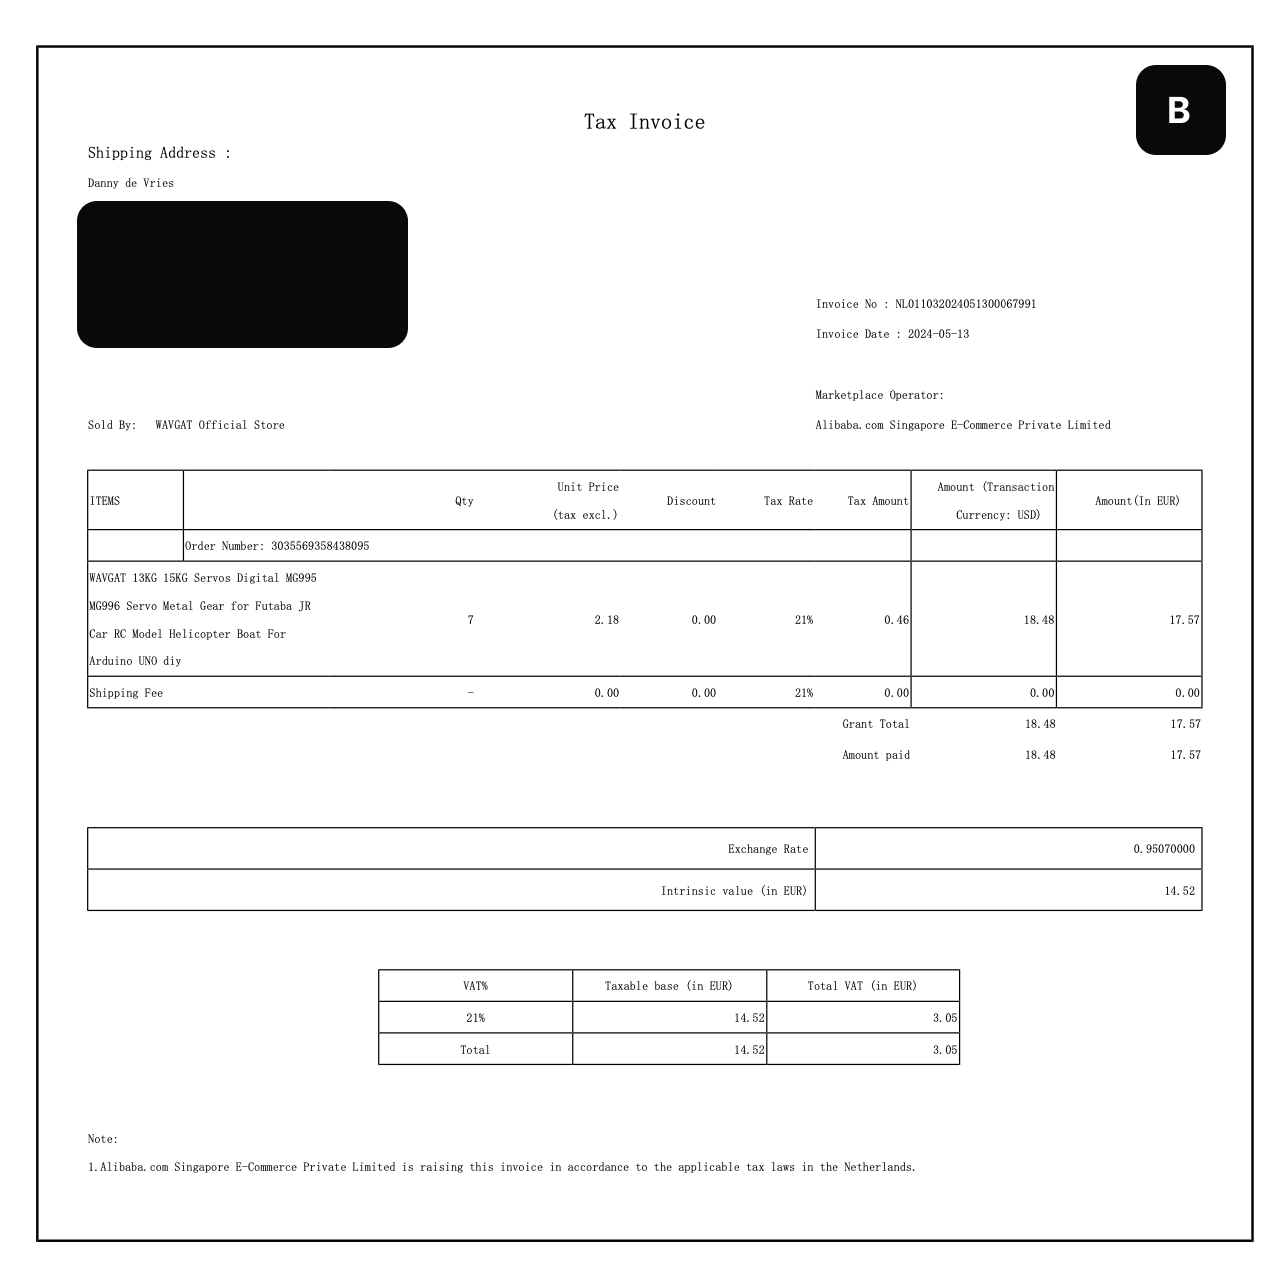
\includegraphics[width=1\textwidth]{servo_motors.jpg}
    \caption{B) Invoice from Alibaba for the Servo Motors}
    \label{fig:mesh1}
\end{figure}

\begin{figure}[h]
    \centering
    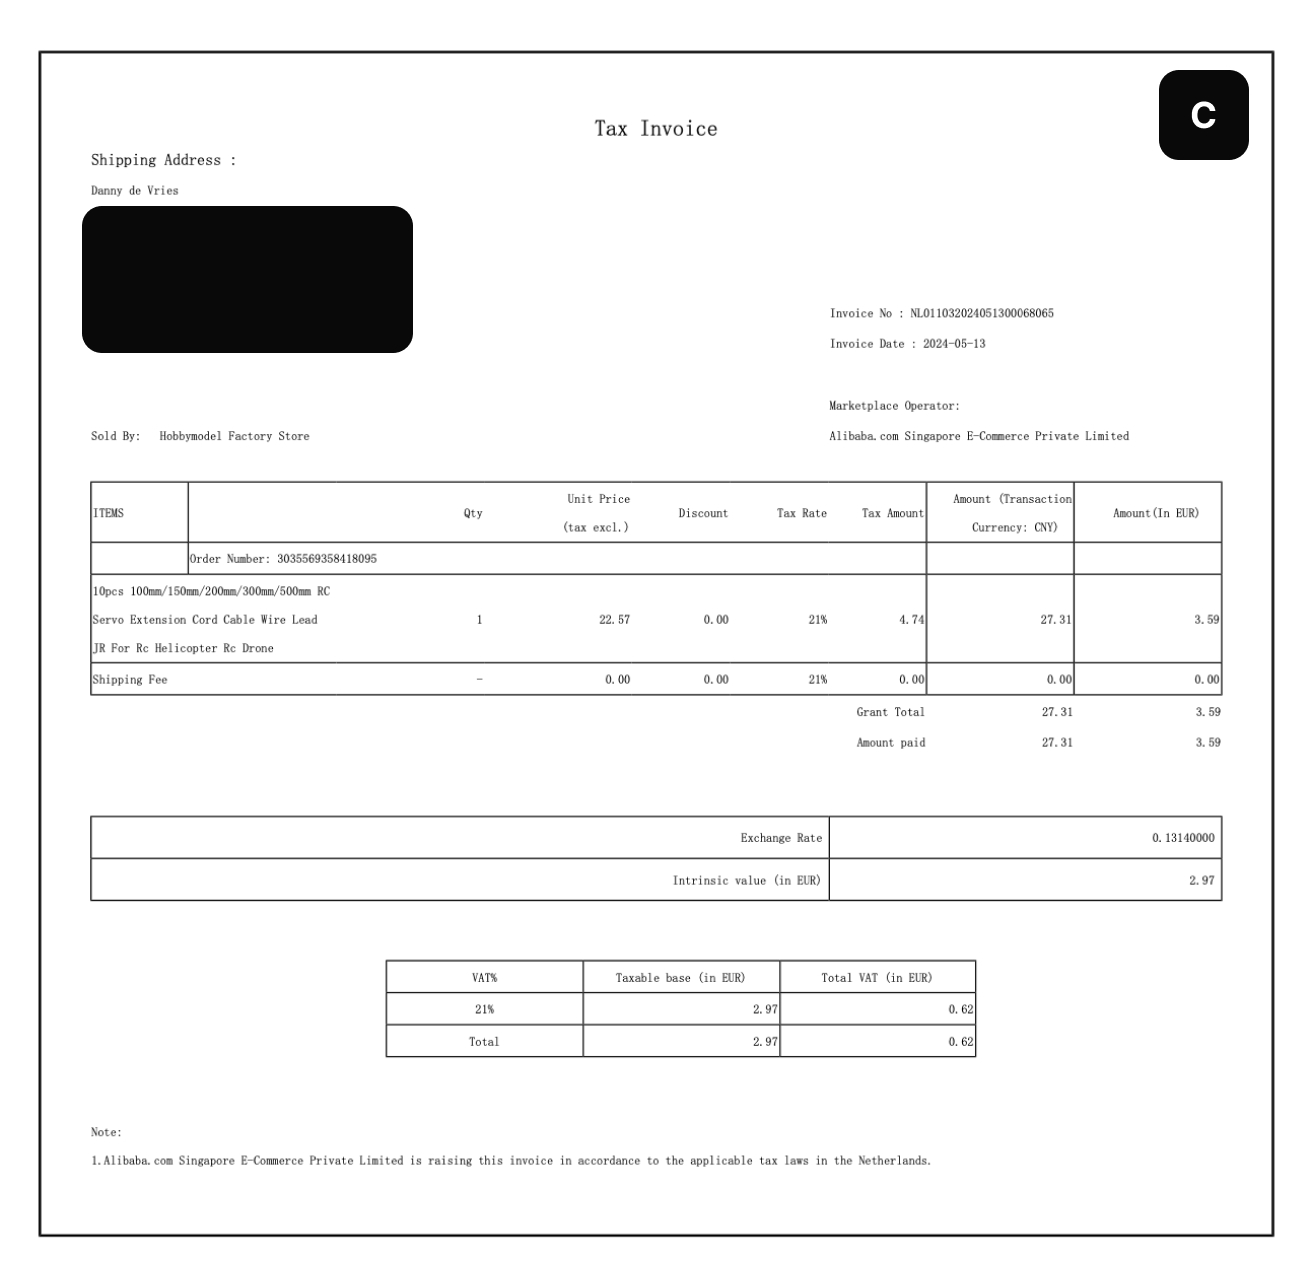
\includegraphics[width=1\textwidth]{extension_cables.jpg}
    \caption{C) Invoice from Alibaba for the Servo Motor extension cables}
    \label{fig:mesh1}
\end{figure}

\begin{figure}[h]
    \centering
    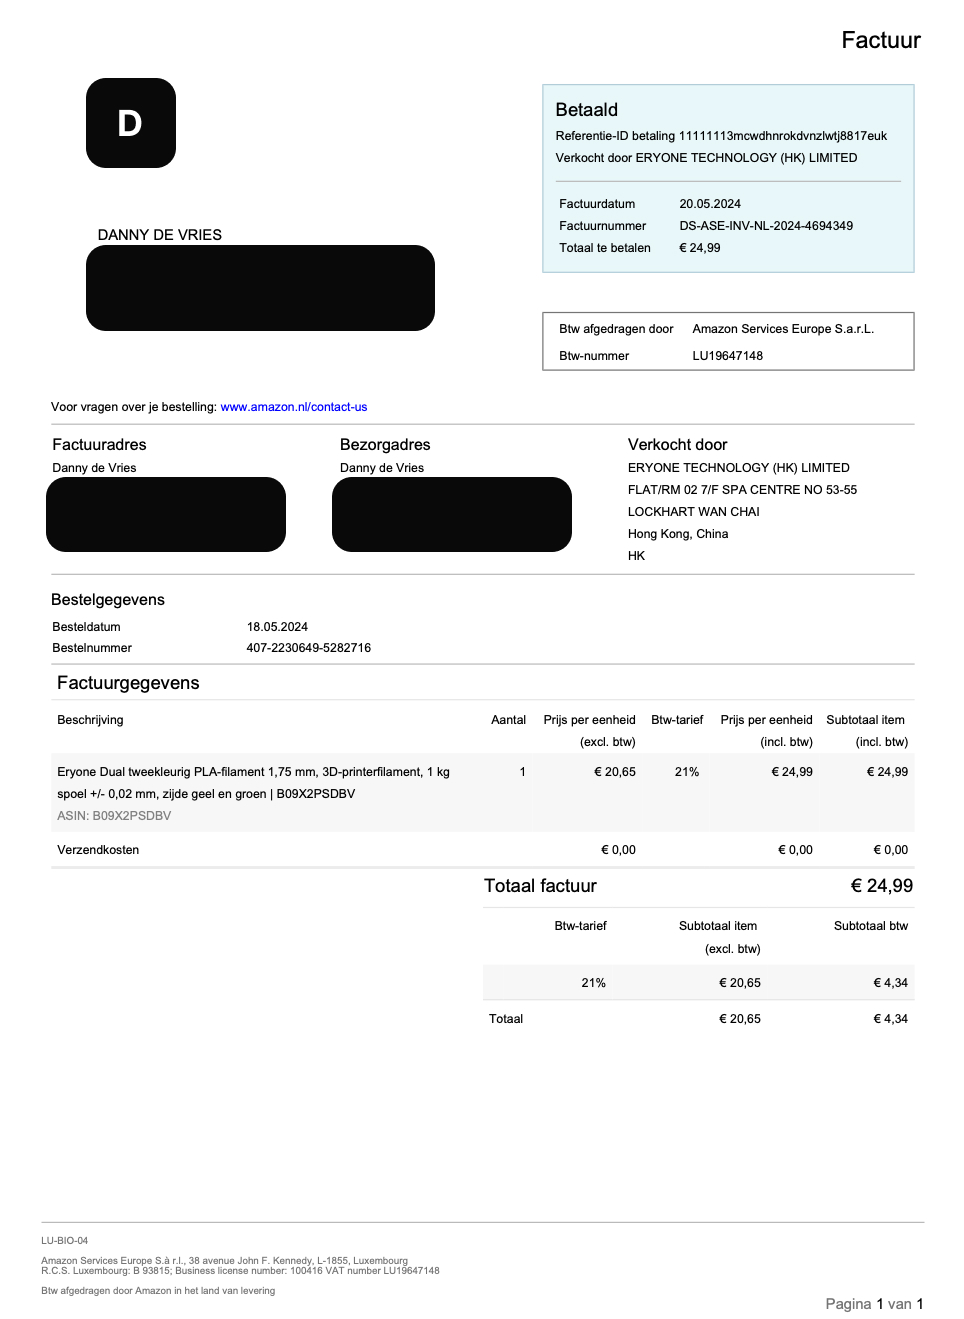
\includegraphics[width=1\textwidth]{filament_pla.jpg}
    \caption{D) Invoice from Amazon for the 3D Printing PLA filament}
    \label{fig:mesh1}
\end{figure}

\begin{figure}[h]
    \centering
    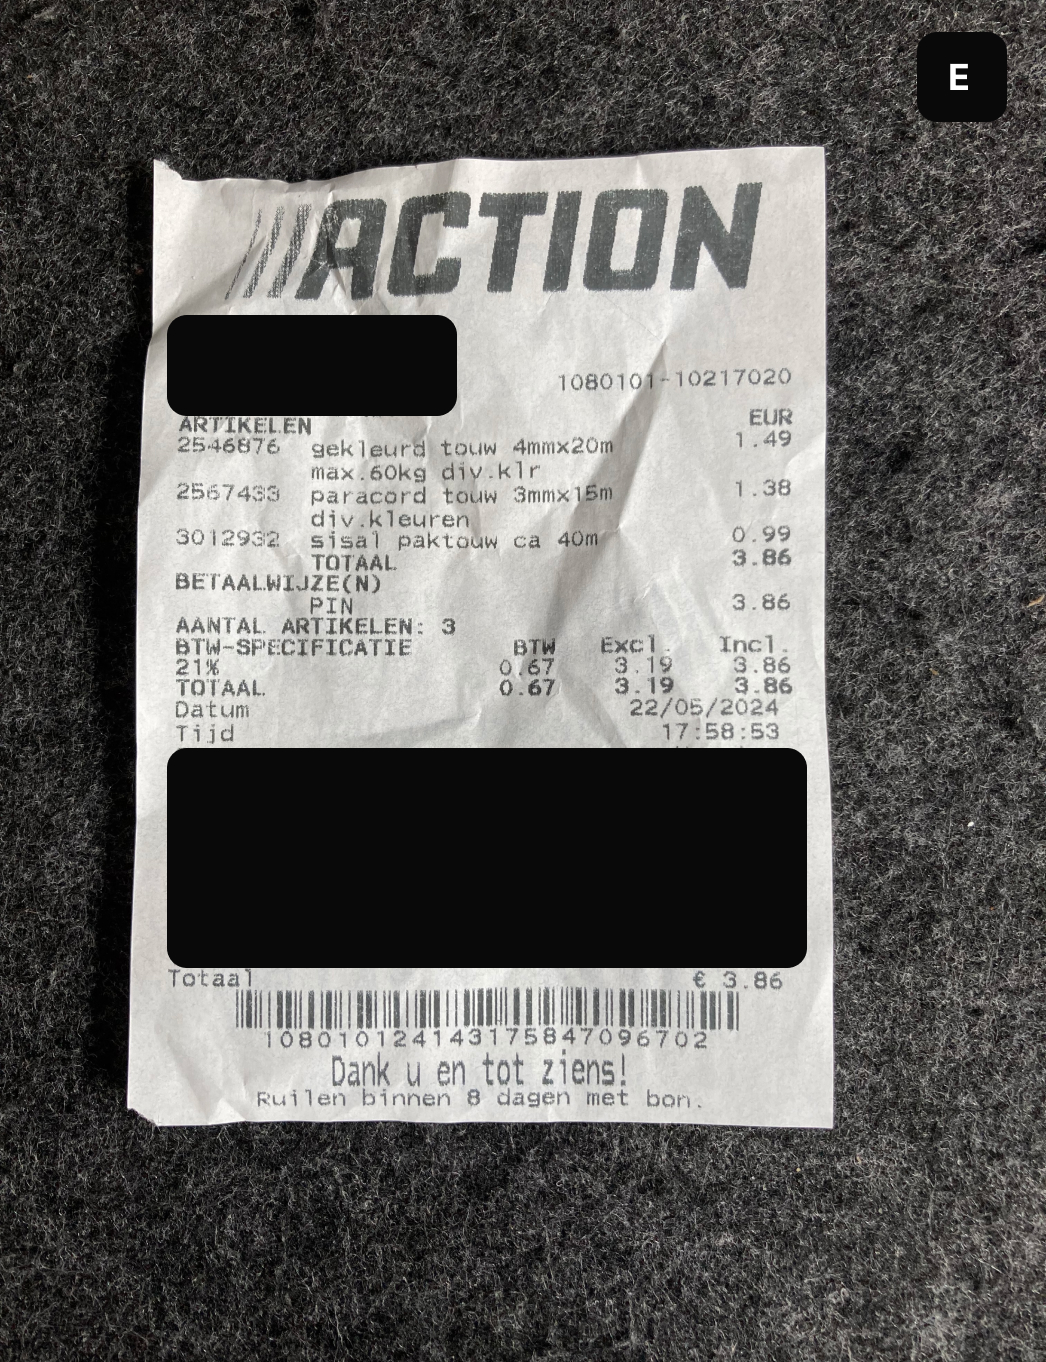
\includegraphics[width=1\textwidth]{ropes.jpg}
    \caption{E) Receipt from Action for the rope strings}
    \label{fig:mesh1}
\end{figure}

\begin{figure}[h]
    \centering
    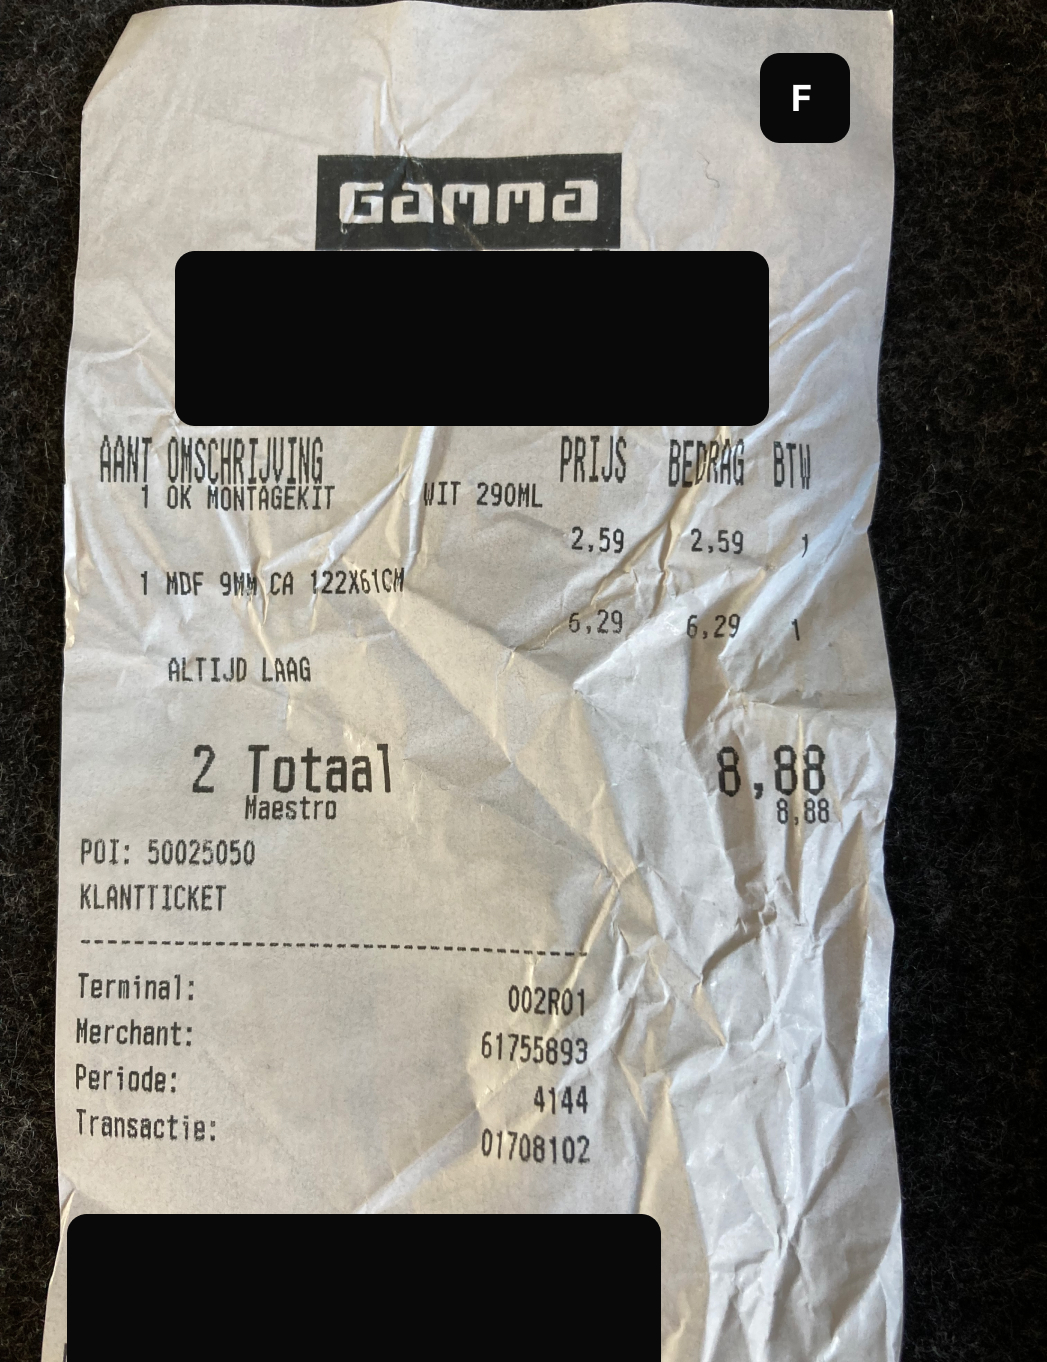
\includegraphics[width=1\textwidth]{wood.jpg}
    \caption{F) Receipt from Gamma for the wooden board and mounting kit}
    \label{fig:mesh1}
\end{figure}

\end{document}